\documentclass[polish,12pt,twoside,a4paper]{report}

\usepackage[a4paper,twoside,left=2.0cm,right=1.5cm,top=1.5cm,bottom=1.5cm]{geometry}
\usepackage[T1]{fontenc}
%\usepackage[cp1250]{inputenc}
\usepackage[utf8]{inputenc}
\usepackage[polish]{babel}
\usepackage{amsmath}
\usepackage{amsfonts}
\usepackage{graphicx}
\usepackage{graphics}
\usepackage{times}
\usepackage{indentfirst}%wciecia a nowych akapitach
\usepackage{float}
\selectlanguage{polish}

%szerokoœœ wciêæ
\setlength{\parindent}{1.25cm}

%numeracja stron
\usepackage{fancyhdr}
\pagestyle{fancy}
\fancyhf{} % usun biezace ustawienia pagin
\fancyhead[LE,RO]{ }
\fancyhead[LO]{ }
\fancyhead[RE]{ }
\fancyfoot[LE,RO]{\small\thepage}
\fancyfoot[LO]{ }
\fancyfoot[RE]{ }
\renewcommand{\headrulewidth}{0.0pt}
\renewcommand{\footrulewidth}{0.0pt}
\addtolength{\headheight}{0.0pt} % pionowy odstep na kreske
\fancypagestyle{plain}{%
\fancyhead{} % usun p. górne na stronach pozbawionych
% numeracji (plain)
\renewcommand{\headrulewidth}{0.0pt} % pozioma kreska
}

\usepackage{color}

\definecolor{greenyellow}   {cmyk}{0.15, 0   , 0.69, 0   }
\definecolor{yellow}        {cmyk}{0   , 0   , 1   , 0   }
\definecolor{goldenrod}     {cmyk}{0   , 0.10, 0.84, 0   }
\definecolor{dandelion}     {cmyk}{0   , 0.29, 0.84, 0   }
\definecolor{apricot}       {cmyk}{0   , 0.32, 0.52, 0   }
\definecolor{peach}         {cmyk}{0   , 0.50, 0.70, 0   }
\definecolor{melon}         {cmyk}{0   , 0.46, 0.50, 0   }
\definecolor{yelloworange}  {cmyk}{0   , 0.42, 1   , 0   }
\definecolor{orange}        {cmyk}{0   , 0.61, 0.87, 0   }
\definecolor{burntorange}   {cmyk}{0   , 0.51, 1   , 0   }
\definecolor{bittersweet}   {cmyk}{0   , 0.75, 1   , 0.24}
\definecolor{redorange}     {cmyk}{0   , 0.77, 0.87, 0   }
\definecolor{mahogany}      {cmyk}{0   , 0.85, 0.87, 0.35}
\definecolor{maroon}        {cmyk}{0   , 0.87, 0.68, 0.32}
\definecolor{brickred}      {cmyk}{0   , 0.89, 0.94, 0.28}
\definecolor{red}           {cmyk}{0   , 1   , 1   , 0   }
\definecolor{orangered}     {cmyk}{0   , 1   , 0.50, 0   }
\definecolor{rubinered}     {cmyk}{0   , 1   , 0.13, 0   }
\definecolor{wildstrawberry}{cmyk}{0   , 0.96, 0.39, 0   }
\definecolor{salmon}        {cmyk}{0   , 0.53, 0.38, 0   }
\definecolor{carnationpink} {cmyk}{0   , 0.63, 0   , 0   }
\definecolor{magenta}       {cmyk}{0   , 1   , 0   , 0   }
\definecolor{violetred}     {cmyk}{0   , 0.81, 0   , 0   }
\definecolor{rhodamine}     {cmyk}{0   , 0.82, 0   , 0   }
\definecolor{mulberry}      {cmyk}{0.34, 0.90, 0   , 0.02}
\definecolor{redviolet}     {cmyk}{0.07, 0.90, 0   , 0.34}
\definecolor{fuchsia}       {cmyk}{0.47, 0.91, 0   , 0.08}
\definecolor{lavender}      {cmyk}{0   , 0.48, 0   , 0   }
\definecolor{thistle}       {cmyk}{0.12, 0.59, 0   , 0   }
\definecolor{orchid}        {cmyk}{0.32, 0.64, 0   , 0   }
\definecolor{darkorchid}    {cmyk}{0.40, 0.80, 0.20, 0   }
\definecolor{purple}        {cmyk}{0.45, 0.86, 0   , 0   }
\definecolor{plum}          {cmyk}{0.50, 1   , 0   , 0   }
\definecolor{violet}        {cmyk}{0.79, 0.88, 0   , 0   }
\definecolor{royalpurple}   {cmyk}{0.75, 0.90, 0   , 0   }
\definecolor{blueviolet}    {cmyk}{0.86, 0.91, 0   , 0.04}
\definecolor{periwinkle}    {cmyk}{0.57, 0.55, 0   , 0   }
\definecolor{cadetblue}     {cmyk}{0.62, 0.57, 0.23, 0   }
\definecolor{cornflowerblue}{cmyk}{0.65, 0.13, 0   , 0   }
\definecolor{midnightblue}  {cmyk}{0.98, 0.13, 0   , 0.43}
\definecolor{navyblue}      {cmyk}{0.94, 0.54, 0   , 0   }
\definecolor{royalblue}     {cmyk}{1   , 0.50, 0   , 0   }
\definecolor{blue}          {cmyk}{1   , 1   , 0   , 0   }
\definecolor{cerulean}      {cmyk}{0.94, 0.11, 0   , 0   }
\definecolor{cyan}          {cmyk}{1   , 0   , 0   , 0   }
\definecolor{processblue}   {cmyk}{0.96, 0   , 0   , 0   }
\definecolor{skyblue}       {cmyk}{0.62, 0   , 0.12, 0   }
\definecolor{turquoise}     {cmyk}{0.85, 0   , 0.20, 0   }
\definecolor{tealblue}      {cmyk}{0.86, 0   , 0.34, 0.02}
\definecolor{aquamarine}    {cmyk}{0.82, 0   , 0.30, 0   }
\definecolor{bluegreen}     {cmyk}{0.85, 0   , 0.33, 0   }
\definecolor{emerald}       {cmyk}{1   , 0   , 0.50, 0   }
\definecolor{junglegreen}   {cmyk}{0.99, 0   , 0.52, 0   }
\definecolor{seagreen}      {cmyk}{0.69, 0   , 0.50, 0   }
\definecolor{green}         {cmyk}{1   , 0   , 1   , 0   }
\definecolor{forestgreen}   {cmyk}{0.91, 0   , 0.88, 0.12}
\definecolor{pinegreen}     {cmyk}{0.92, 0   , 0.59, 0.25}
\definecolor{limegreen}     {cmyk}{0.50, 0   , 1   , 0   }
\definecolor{yellowgreen}   {cmyk}{0.44, 0   , 0.74, 0   }
\definecolor{springgreen}   {cmyk}{0.26, 0   , 0.76, 0   }
\definecolor{olivegreen}    {cmyk}{0.64, 0   , 0.95, 0.40}
\definecolor{rawsienna}     {cmyk}{0   , 0.72, 1   , 0.45}
\definecolor{sepia}         {cmyk}{0   , 0.83, 1   , 0.70}
\definecolor{brown}         {cmyk}{0   , 0.81, 1   , 0.60}
\definecolor{tan}           {cmyk}{0.14, 0.42, 0.56, 0   }
\definecolor{gray}          {cmyk}{0   , 0   , 0   , 0.50}
\definecolor{black}         {cmyk}{0   , 0   , 0   , 1   }
\definecolor{white}         {cmyk}{0   , 0   , 0   , 0   } 


\newcommand{\wydzial}{KOLEGIUM INFORMATYKI STOSOWANEJ}
\newcommand{\kierunek}{Kierunek: INFORMATYKA}
\newcommand{\specjalnosc}{Specjalność: Teleinformatyka}
\newcommand{\autor}{Kamil Dudek}
\newcommand{\album}{Nr albumu studenta w68560}
\newcommand{\temat}{Program "Sklep"}
\newcommand{\promotor}{dr inż. Janusz Korniak}
\newcommand{\typpracy}{PRACA DYPLOMOWA INŻYNIERSKA}
\newcommand{\miasto}{Rzeszów}
\newcommand{\rok}{2024}

\begin{document}

\noindent
\parbox{65mm}{
\includegraphics[width=13.0cm, height=3.0cm]{logoWSIiZ}}

\vspace{10mm}
\begin{center}
{\Large{}\textbf{\wydzial}}
\end{center}
\vspace{10mm}
\noindent
\hspace{30mm}{\Large{}\textbf{\kierunek}}\\

\noindent
\hspace{30mm}{\Large{}\textbf{\specjalnosc}}
\vspace{30mm}
\begin{center}
	{\large{}\autor}\\
	{\large{}\album}\\
	\vspace{15pt}
	{\huge{}\textbf{\textit{\temat}}}\\
	\vspace{20pt}
	{\normalsize{}Promotor: \promotor}\\
	\vspace{100pt}
	{\LARGE{}\textbf{\typpracy}}\\
	\vspace{190pt}
	{\large{}\textbf{\miasto {} \rok}}
\end{center}

\thispagestyle{empty}
\newpage

\tableofcontents
\thispagestyle{empty}
\newpage

\chapter*{Opis założeń projektu}

Program będzie aplikacją konsolową napisaną w języku C\#. Głównym celem projektu będzie prowadzenie działaności sprzedaży ubrań. Obsługiwał on będzie funkcjonalność zarówno od strony klienta jak i sprzedawcy. Klient będzie mógł przeglądać dostępne towary, a następnie wybierać i dodawać do koszyka te, które zechce kupić w wybranym rozmiarze i ilości. Ponadto będzie też możliwość sortowania, filtrowania oraz grupowania produktów po cenie. Wszystko to, aby ułatwić klientowi wybór, a sprzedawcy pracę.\newline

Sprzedawca będzie mógł dodawać nowe towary do bazy danych zarówno ręcznie jak i importując produkty z pliku csv. Możliwy będzie również eksport produktów do pliku csv. Dzięki bazie danych Sql, dane będą przechowywane w bezpieczny sposób, a pobieranie ich oraz modyfikacja w trakcie działania programu będzie szybka i wygodna.

\addcontentsline{toc}{chapter}{Opis założeń projektu}
\newpage
\chapter{Wymagania projektu}
\section{Wymagania funkcjonalne}
Wymagania funkcjonalne definiują zbiór działań i funkcji, które system powinien realizować, aby spełnić określone cele biznesowe. W przypadku projektu konsolowego sklepu w języku C\#, wymagania funkcjonalne obejmują szereg operacji związanych zarówno z zarządzaniem produktami, jak i obsługą zamówień.

\subsection{Zarządzanie produktami}
System umożliwia dodawanie nowych produktów do bazy danych poprzez interfejs konsolowy. Podczas dodawania produktu należy podać jego nazwę, cenę, ilość na stanie oraz inne istotne informacje. Sprzedawca ma możliwość edycji istniejących produktów, w tym zmiany nazwy, ceny, ilości na stanie itp. Zmiany dokonane na produkcie powinny być odzwierciedlone w bazie danych sklepu. System umożliwia usunięcie produktów z bazy danych. Usunięcie produktu powinno być potwierdzone przez użytkownika, aby zapobiec przypadkowemu usunięciu istotnych danych.

\subsection{Zarządzanie zamówieniami}
Klienci mogą przeglądać dostępne produkty i dodać je do koszyka zakupowego. System umożliwia składanie zamówień poprzez interaktywny interfejs konsolowy, gdzie klient może zobaczyć sumaryczną kwotę zamówienia. Użytkownicy mogą edytować zawartość swojego koszyka, zmieniając ilość produktów lub usuwając je.
W przypadku zmian w zamówieniu, system powinien na bieżąco aktualizować wartość zamówienia. Klient może zatwierdzić i złożyć zamówienie, co powinno spowodować zapisanie zamówienia w bazie danych.

\subsection{Autoryzacja i uwierzytelnianie}
System umożliwia klientom logowanie do swojego konta lub rejestrację nowego konta w celu dokonywania zakupów. Użytkownicy mogą mieć różne poziomy dostępu w systemie, np. klient, sprzedawca, co wpływa na dostępne funkcje. Wyboru rodzaju konta należy dokonać przy włączeniu aplikacji.

\newpage
\section{Wymagania niefunkcjonalne}
Wymagania niefunkcjonalne definiują cechy systemu, które nie są związane bezpośrednio z jego funkcjonalnością, ale mają istotne znaczenie dla jego jakości, wydajności, bezpieczeństwa czy użyteczności. Poniżej przedstawione są główne wymagania niefunkcjonalne dla projektu konsolowego sklepu.

\subsection{Wydajność}
System powinien reagować na interakcje użytkownika w sposób szybki i płynny, zapewniając czas odpowiedzi poniżej 1 sekundy dla podstawowych operacji. Aplikacja powinna efektywnie zarządzać zasobami, takimi jak pamięć i procesor, minimalizując zużycie zasobów systemowych.

\subsection{Bezpieczeństwo}
System powinien zapewnić mechanizmy autoryzacji i uwierzytelniania użytkowników, aby zapobiec nieautoryzowanemu dostępowi do danych. W zależności od roli w systemie użytkownik będzie miał dostęp tylko do swoich funkcjonalności. Dane użytkowników (takie jak dane osobowe i hasło) powinny być przechowywane w sposób bezpieczny, zapewniający poufność i integralność.

\subsection{Użyteczność}
Interfejs konsolowy powinien być przejrzysty i intuicyjny, umożliwiając użytkownikom łatwe korzystanie z funkcji sklepu. Komunikaty o błędach powinny być czytelne i informatywne, aby użytkownicy mogli łatwo zrozumieć przyczyny problemów i podjąć odpowiednie działania naprawcze.
\newpage
\chapter{Opis struktury projektu}
Diagram klas reprezentuje schemat powiązań pomiędzy klasami i encjami w bazie danych. Pola, które znajdują się w tabelach, są właściwościami w klasach i zawierać będą wartości, które będą zapisane w bazie. Na łączeniach pomiędzy tabelami widać rodzaj relacji.
\section{Diagram klas}
\begin{figure}[!ht]
	\centering
		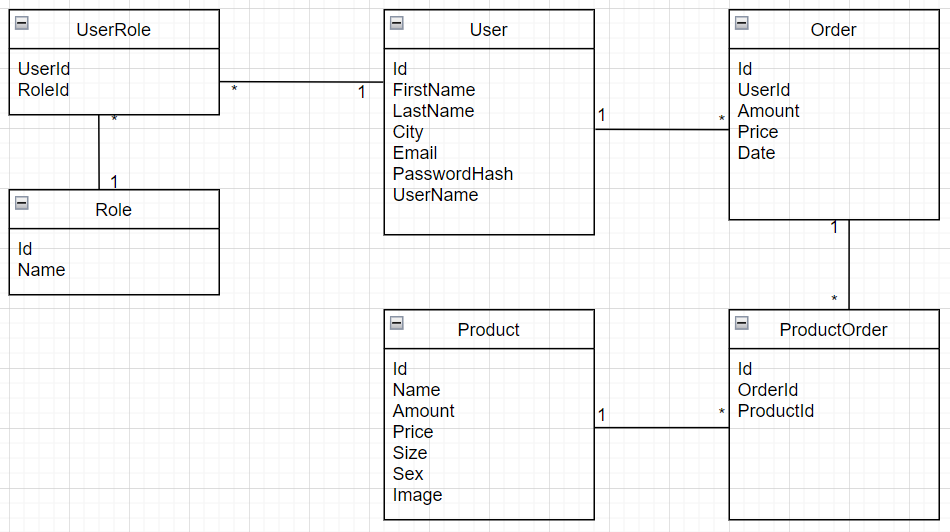
\includegraphics[width=15cm]{diagram.png}
	\caption{\footnotesize Diagram klas programu Sklep}
	\label{fig:plotend}
\end{figure}

Powyższy diagram przedstawia klasy, które reprezentują dane użytkownika, produktów oraz zamówień. Klasy odpowiadające na dane klienta oraz role w systemie zostaną wygenerowane przez bibliotekę Identity, która służy do autoryzacji i autentykacji użytkowników. Udostępnia ona również gotowe mechanizmy logowania, rejestracji i wiele innych. Użytkownik połączony jest z rolą w relacji wiele do wielu, dlatego też istnieje klasa łącząca UserRole.\newline

W takiej samej relacji znajdują się klasa Product oraz Order. Jeden produkt może znajdować się w wielu zamówieniach i tak samo jedno zamówienie może zawierać wiele produktów, przez co w tym przypadku również zastosowano powiązanie poprzez klasę łączącą. Użytkownik może mieć wiele zamówień w sklepie, a jedno zamówienie przypisane jest tylko do jednego klienta, przez co połączony jest w relacji jeden do wielu.\newline

Klasa użytkownika zawiera podstawowe informacje o kliencie, poprzez które będzie można go zweryfikować. Produkt zawiera informacje takie jak nazwa, ilość sztuk dostępna w sklepie, cena za sztukę, rozmiar, płeć, oraz obrazek, który w formie ascii artu będzie przedstawiał dany artykuł na konsoli. Natomiast tabela Order przechywać będzie dane o zamówieniu takie jak kto i kiedy złozył zamówienie ilość produktów oraz całkowita kwota zamówienia.
\newpage
\chapter{Opis techniczny projektu}
\section{Wykorzystana technologia}

Projekt sklepu to aplikacja konsolowa napisana w języku C\#. Jej głównym założeniem jest podział funkcjonalności, na te które są w uprawnieniach sprzedawcy, a także, 
te do których dostęp ma klient. Obsługa menu programu polega na przechodzeniu pomiędzy opcjami przy pomocy strzałek co ułatwia korzystanie z interface'u.\newline

W celu uatrakcyjnienia wyglądu, użyto kolorowania składni oraz obrazków reprezentujących produkty sklepu odzieżowego przy pomocy ASCII art. Mechanizm koszyka, do którego klient
może dodawac wybrane produkty, aby później móc je kupić zaimplementowano korzystając z klasy statycznej. Przy pomocy polecenia \textit{Console.SetCursorPosition(y, x)} zmieniane są miejsca
kursora na konsoli, dzięki czemu pisanie tekstu można było zaczynać z dowolnego miejsca.\newline

Głównym elementem programu, który został wykorzystany wielokrotnie przy każdorazowym przejściu do kolejnego menu była pętla while. We wspomnianej pętli wyświetlane zostały menu, tak długo, aż spełniony został warunek przerwania, który zachodził, gdy zaznaczona, a następnie zatwierdzona została opcja \textit{Wyjście}.\newline

Aby zapewnić w aplikacji korzystanie z tych samych danych, które znajdowały się podczas ostatniego użytkownia przed jej zamknięciem, zastosowano bazę danych SQL. Jest to relacyjna baza danych, która przechowuje informacje w relacji między tabelami. W tym celu zainstalowano bibliotekę EntityFrameworkCore, w wersji 6, która kompatybilna jest z również 6 wersją .NET, który wykorzystany został do stworzenia danej aplikacji.\newline

Sprzedawca ma możliwość generowania raportu PDF z asortymentu dostępnego w sklepie. Funkcjonalność tą zaimplementowano przy pomocy biblioteki iText7, która specjalizuje się w tworzeniu plików pdf. Do projektu dołączono ją poprzez NuGet.

\section{Baza danych}
W programie klasą odpowiedzialną za konfigurację połączenia bazy danych z aplikacją jest klasa \textit{ApplicationDbContext}. Dziedziczy ona po klasie DbContext, dzięki czemu można nadpisać metodę OnConfiguring. W jej ciele, znajduje się konfiguracja połączenia z lokalną bazą danych podaną w adresie \textit{ConnectionString}. Użyto w niej metodę \textit{UseLazyLoadingProxies}. Dzięki temu, kiedy nastąpi próba dostępu do powiązanych encji, będą one leniwie ładowane, nawet w kontekście asynchronicznym. Co za tym idzie, w modelach, które opisują budowę poszczególnych tabel zastosowano słówko \textit{virtual}, aby zaciągać dane obiektów będąnych w relacji.\newline

Logika działania programu zawarta jest w klauzuli \textit{using}, w której tworzony jest kontekst bazy danych, co umożliwia do nich dostęp. W jej obrębie stworzono obiekty, które reprezentują repozytoria. Każde repozytorium pełni funkcję dostępu do poszczególnych typów danych zawartych w tabelach bazy danych. Oddzielają one kod logiki realizujący operację od dostępu do informacji.
\newpage
\chapter{Harmonogram prac}
\section{Diagram Gantta}

Diagram Gantta to narzędzie wykorzystywane do przedstawiania harmonogramu zadań w czasie. Składa się z osi poziomej reprezentującej czas oraz osi pionowej przedstawiającej zadania. Każde zadanie jest przedstawiane za pomocą prostokąta, a jego długość odpowiada czasowi trwania zadania.\newline

Na diagramie Gantta reprezentującym harmonogram pracy podczas tworzenia aplikacji sklepu znajduje się również legenda, która opisuje kolory użyte do prezentacji zadania. Kolor pomarańczowy reprezentuje prace projektowe oraz analityczne. Zazwyczaj takie prace wykonywane są jako pierwsze jeszcze przed implementacją kodu. Na podstawie ustaleń w tym procesie powstaje architektura projektu.\newline

Kolorem niebieskim oznaczono prace frontowe odpowiadajace za wygląd aplikacji. Najczęściej prace te wykonywane są jednocześnie z pracami backendowymi. Jednak w przypadku aplikacji konsolowej najpierw wykonano prace odpowiadające za wizualną formę programu.\newline

Kolorem zielonym zaznaczono na diagramie prace nad implementacją operacji i mechanizmów logicznych.\newline

\begin{figure}[!ht]
	\centering
		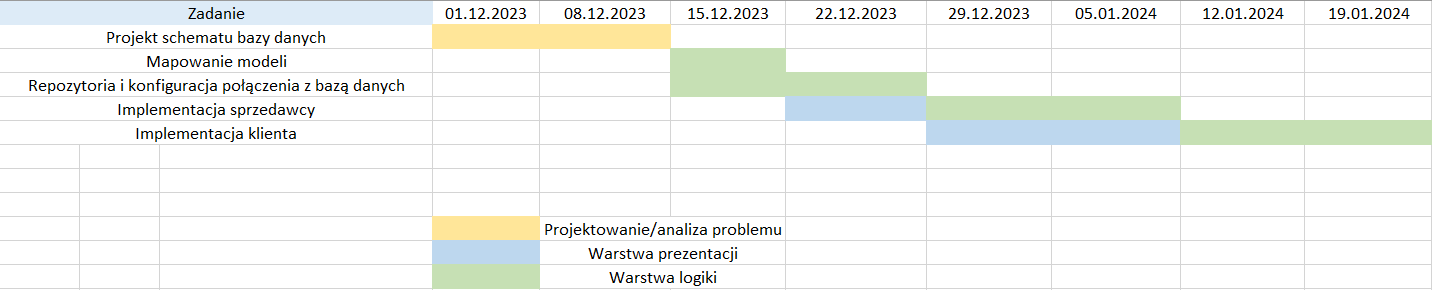
\includegraphics[width=15cm]{gant.png}
	\caption{\footnotesize Diagram Gantta}
	\label{fig:plotend}
\end{figure}
\newpage
\chapter{Repozytorium i system kontroli wersji}

Pliki projektu oraz pliku z dokumentacją, umieszczone zostaly na zdalnym repozytorium kodu pod adresem \href{https://github.com/KamilDudek00/Projekt-programowanie.git}{https://github.com/KamilDudek00/Projekt-programowanie.git}. GitHub to platforma internetowa do hostowania projektów programistycznych, współpracy zespołowej i kontroli wersji przy użyciu systemu kontroli wersji Git. Oferuje narzędzia umożliwiające programistom pracę nad projektami, zarządzanie kodem źródłowym, śledzenie problemów, zarządzanie zadaniem i współpracę z innymi członkami zespołu.\newline 

GitHub jest jednym z najpopularniejszych serwisów hostujących repozytoria Git i jest szeroko używany w społeczności programistycznej do współpracy nad projektami. Z tego miejsca można bezpośrednio pobrać pliki na dysk lub sklonować repozytorium dzięki czemu od razu można zacząć pracę nad kodem i wprowadzać do repozytorium na GitHub.

\begin{figure}[!ht]
	\centering
		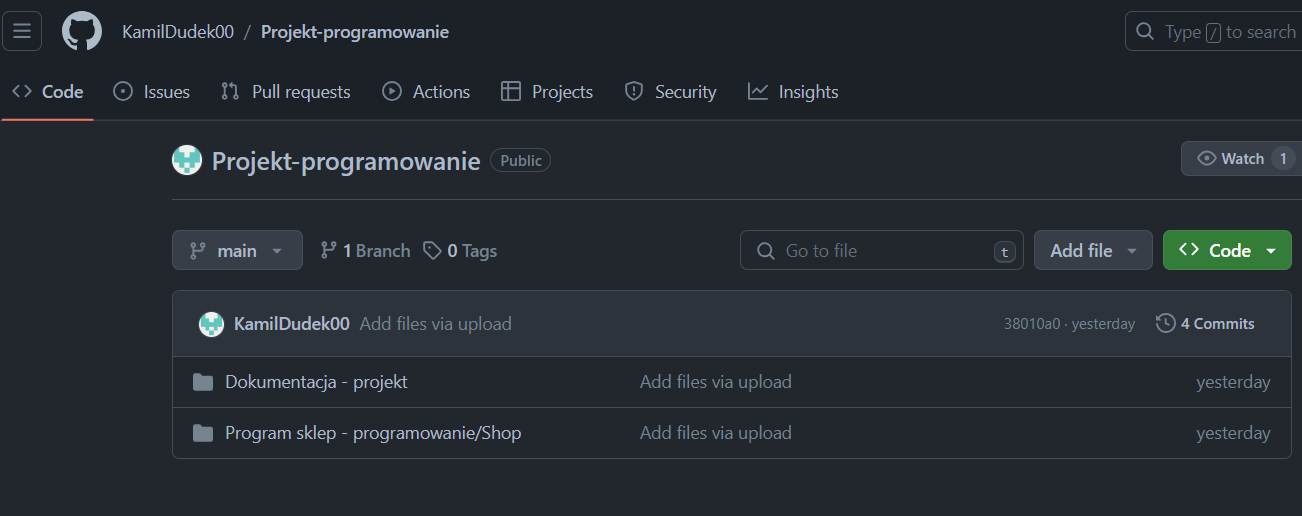
\includegraphics[width=15cm]{screeny/repo.png}
	\caption{\footnotesize Repozytorium z kodem projektu oraz plikami dokumentacji}
	\label{fig:plotend}
\end{figure}
\newpage
\chapter{Prezentacja warstwy użytkowej}
Projekt sklepu został w całości zrealizowany jako aplikacja konsolowa. Oznacza to, że zarówno logika działania programu oraz jej wygląd zostały napisane w języku C\#. Jest to także jednoznaczne z tym, że poruszanie się po programie przez użytkownika odbywa się w konsoli bez dodatkowego interfejsu graficznego, przy pomocy jedynie klawiatury.\newline

Poniżej zostaną przedstawione zrzuty ekranu z najważniejszych funkcjonalności w programie, aby zaprezentować w ten sposób wygląd oraz pogląd działania aplikacji.\newline

Po uruchomieniu aplikacji pierwszym ekranem jest ekran powitalny, który jednocześnie jest miejscem wyboru roli użytkownika, który będzie korzystał z programu. Z programu można korzystać jako sprzedawca lub klient.\newline

\section{Sprzedawca}

\begin{figure}[H]
	\centering
		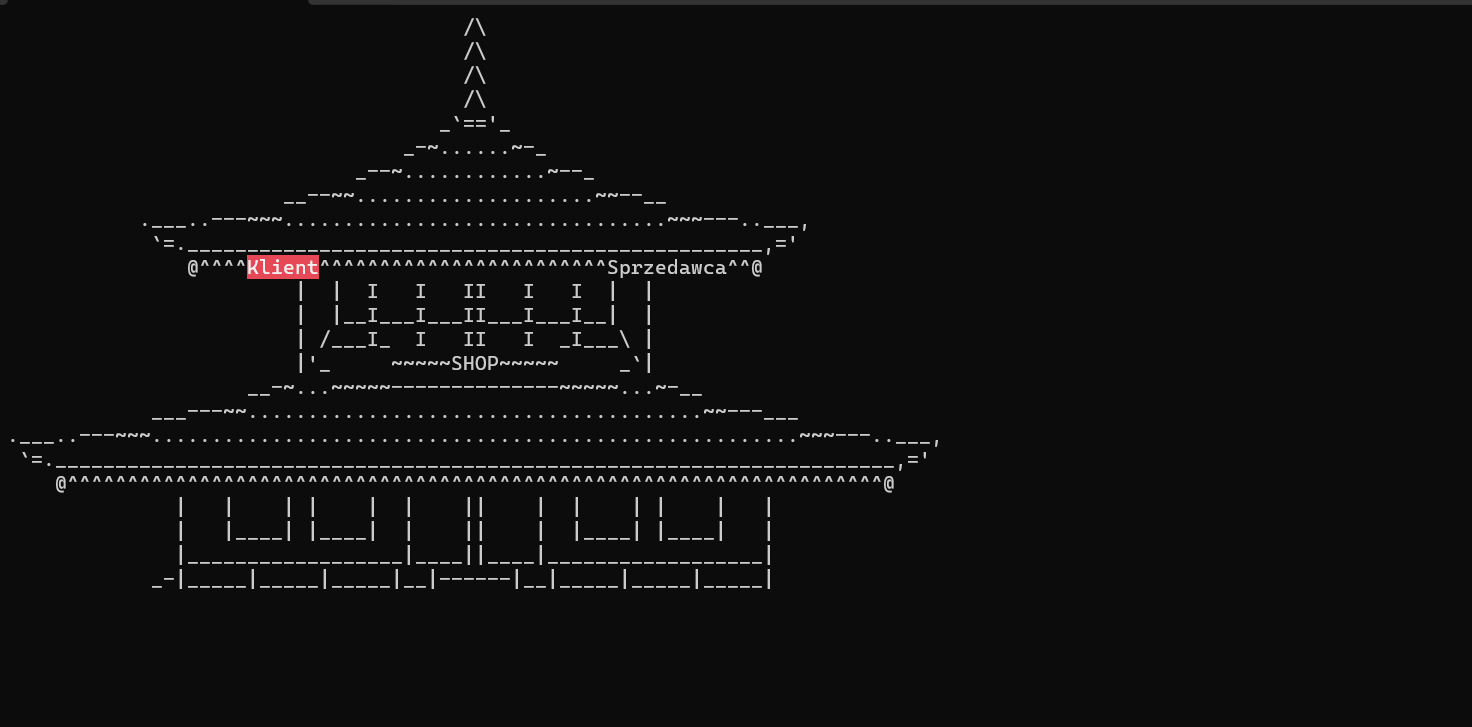
\includegraphics[width=15cm]{screeny/ekran_start.png}
	\caption{\footnotesize Wybór roli użytkownika}
	\label{fig:plotend}
\end{figure}

Po wyborze roli pojawia się ekran, w którym należy zdecydować pomiędzy zalogowaniem się lub rejestracją. Wygląd tych ekranów jest identyczny zarówno dla sprzedawcy jak i klienta. W zależności od wyboru wyświetlają się formularze gdzie kolejno należy podawać kolejne informacje. W przypadku rejestracji w systemie tworzy się konto użytkownika z rolą odpowiadającą wcześniejszemu wyborowi.

\begin{figure}[H]
    \centering
		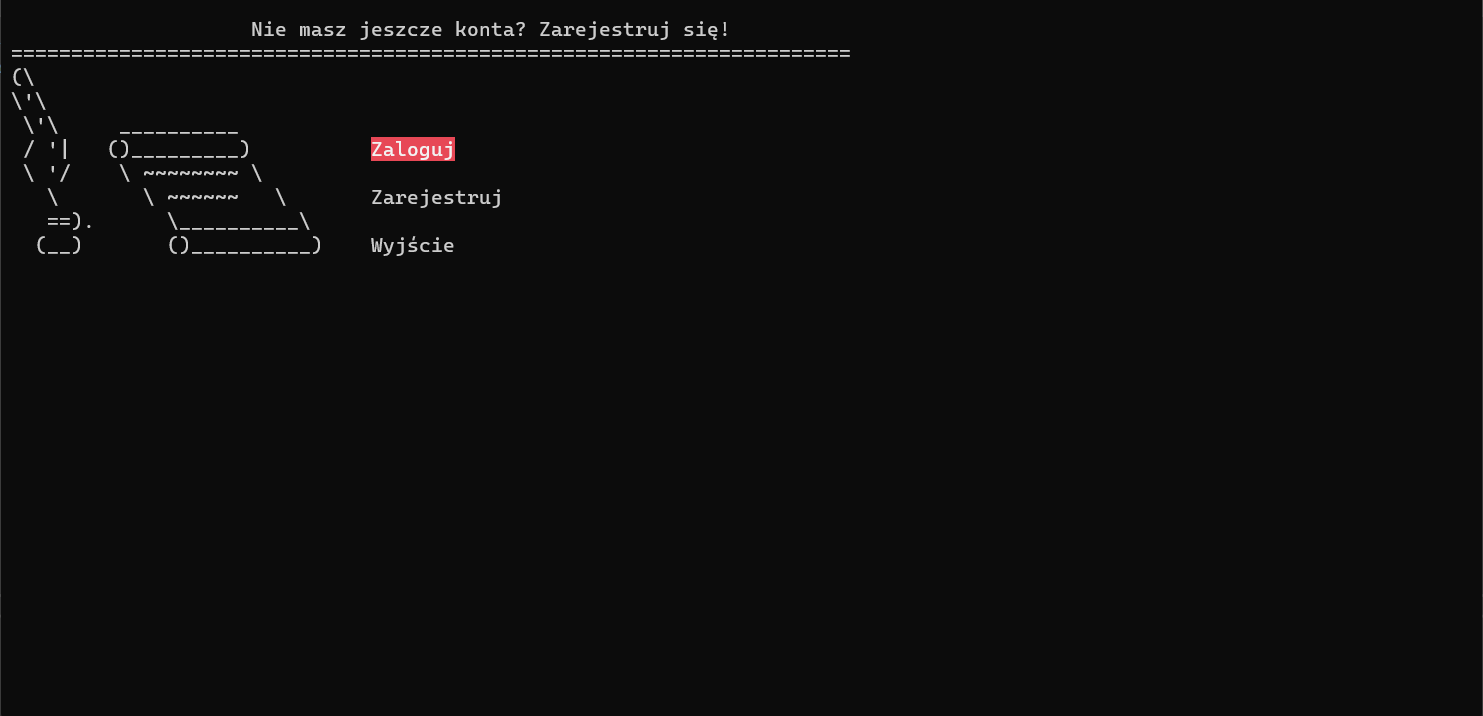
\includegraphics[width=15cm]{screeny/logowanie_sprzedawca.png}
	\caption{\footnotesize Ekran logowania i rejestracji}
	\label{fig:plotend}
\end{figure}

Logując się do aplikacji jako sprzedawca ma on do wyboru opcje widoczne na \textit{Rysunku 5.3}.

\begin{figure}[H]
	\centering
		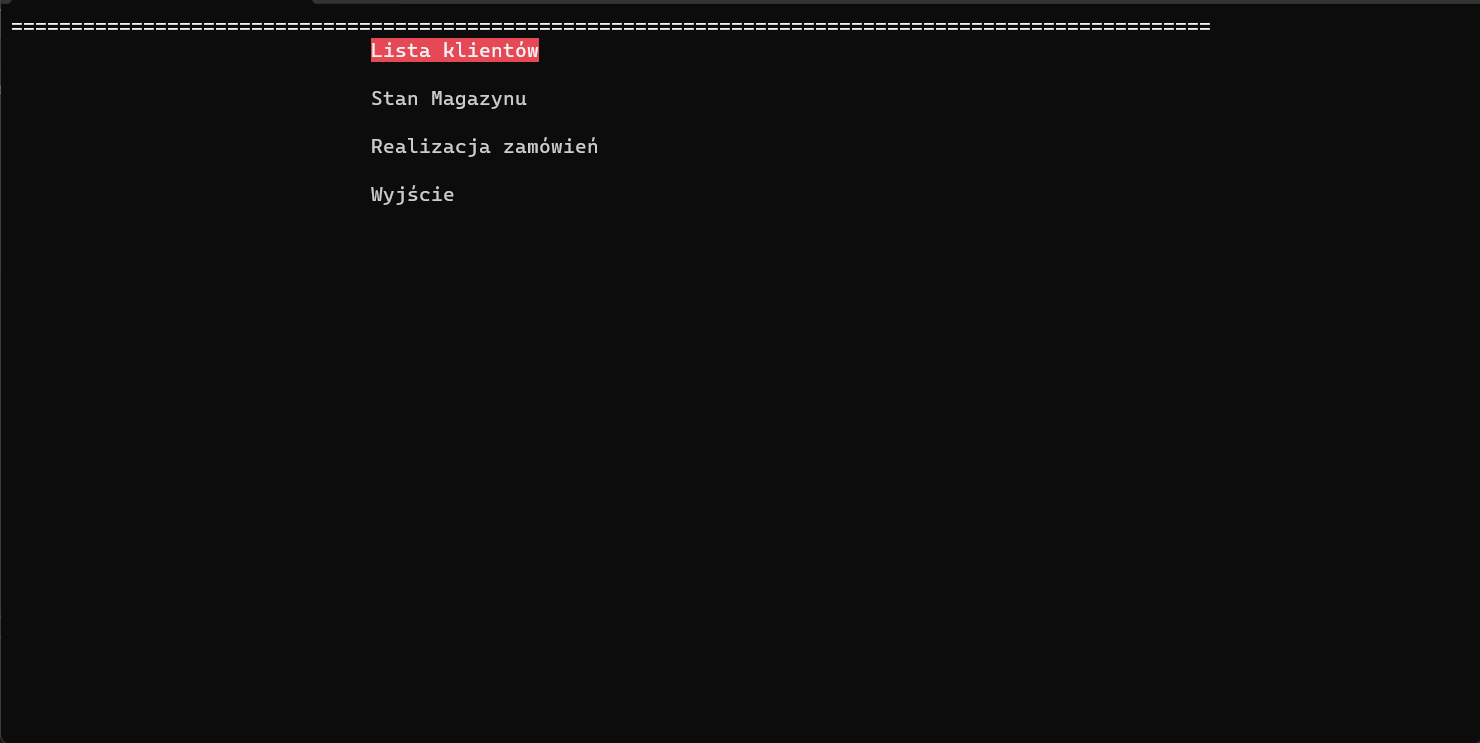
\includegraphics[width=15cm]{screeny/sprzedawca_menu.png}
	\caption{\footnotesize Menu sprzedawcy}
	\label{fig:plotend}
\end{figure}

Po przejściu do opcji \textit{Lista klientów}, sprzedawca ma możliwość usunięcia klienta po adresie e-mail. Na liście wyświetlają się tylko użytkownicy z rolą klienta. Widać ich podstawowe dane personalne oraz liczbę zamówień złożonych w systemie. Ekran ten zaprezentowany został na \textit{Rysunku 5.4}.

\begin{figure}[H]
	\centering
		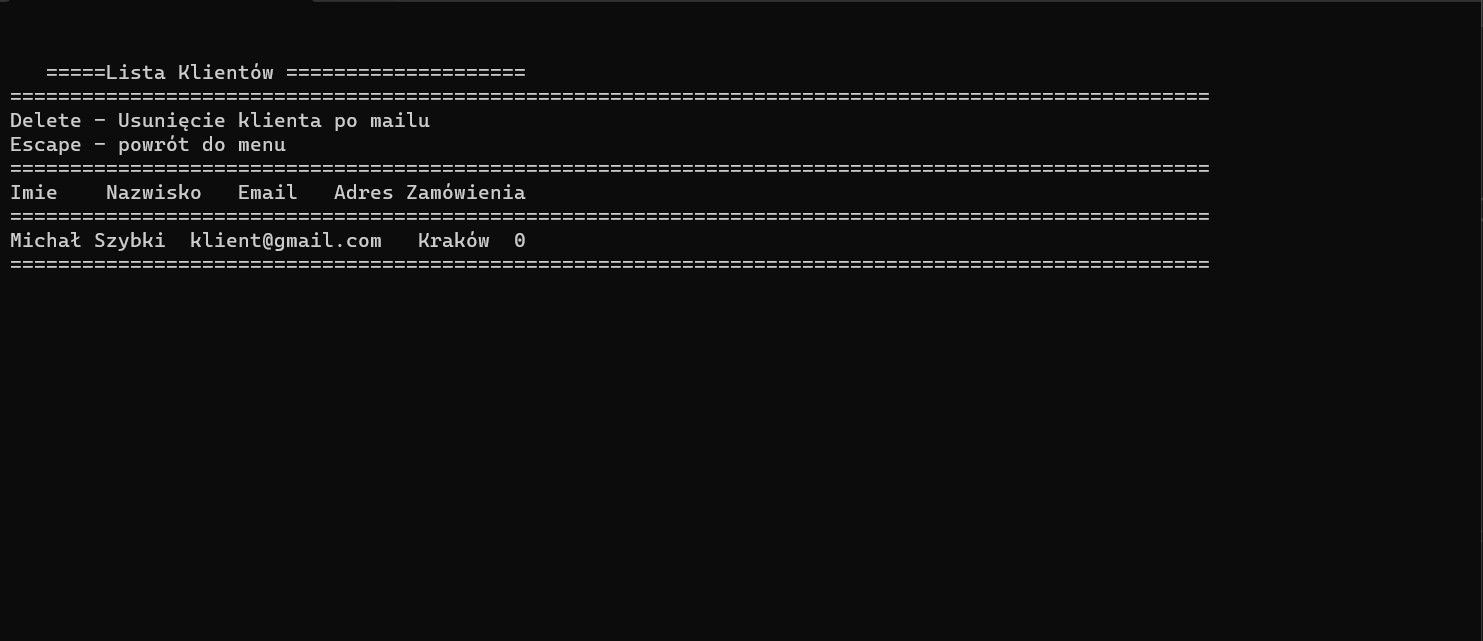
\includegraphics[width=15cm]{screeny/lista_klientow.png}
	\caption{\footnotesize Lista klientów}
	\label{fig:plotend}
\end{figure}

Kolejną możliwą opcją jest wyświetlenie stanu magazynu, czyli wszystkich dostępnych produktów w sklepie. Ponadto, w tym menu można również dodać nowy produkt, usunąć go lub edytować. Możliwe jest również posortowanie na liście produktów po nazwie. Jeśli sprzedawca uzna, że chce na przykład wydrukować daną listę lub ją wyeksportować, ma możliwość wygenerowania pliku pdf z dostępnymi w sklepie towarami.

\begin{figure}[H]
	\centering
		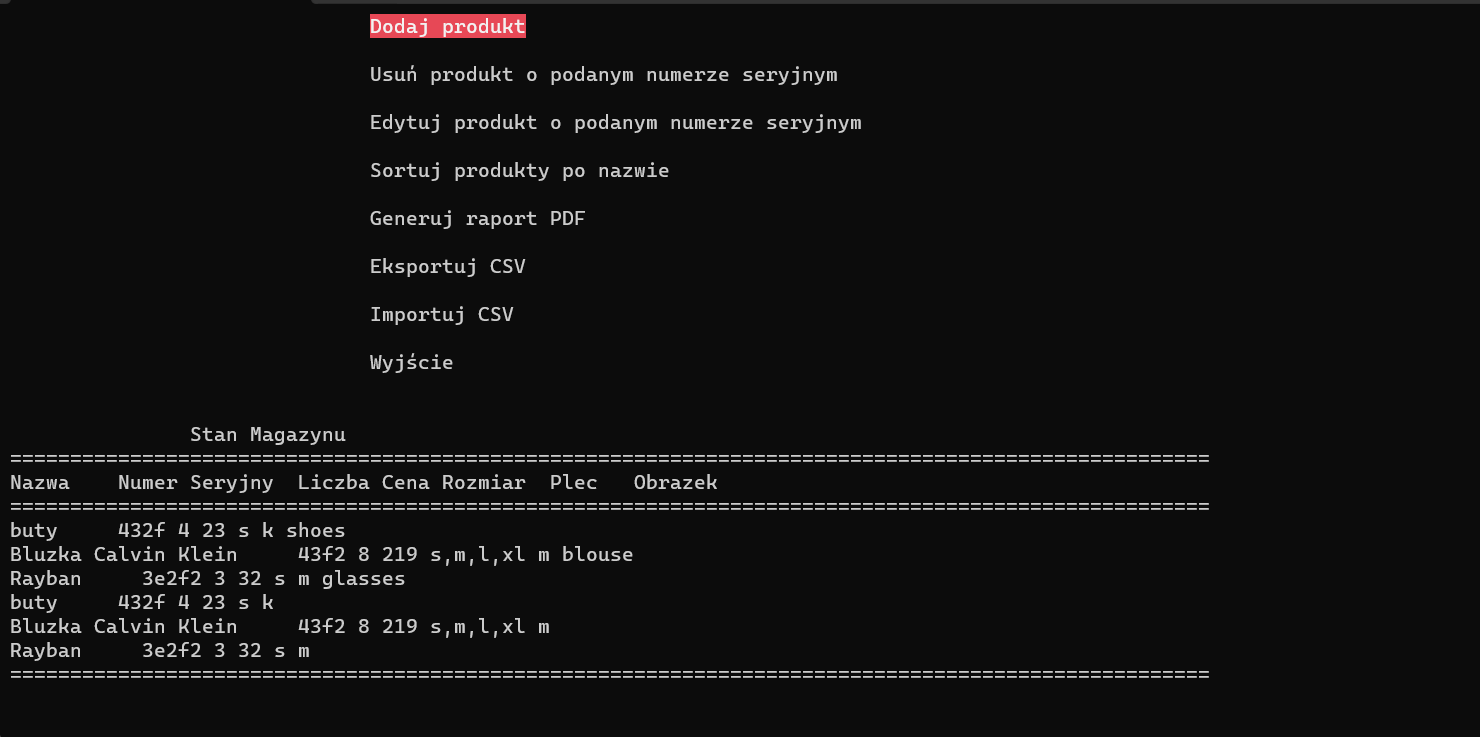
\includegraphics[width=15cm]{screeny/lista_produktow_sprz.png}
	\caption{\footnotesize Menu stan magazynu}
	\label{fig:plotend}
\end{figure}

W otatniej zakładce od strony sprzedawcy, mianowicie \textit{Realizacja zamówień}, wyświetlane są wszystkie zamówienia w systemie zarówno te zrealizowane jak i te, które dopiero zostały złożone. Sprzedawca może usunąć wybrane zamówienie z listy zamówień lub zrealizować zamówienie. Metoda ta zmienia status zamówienia z \textit{złożone} na \textit{zrealizowane}.

\begin{figure}[H]
	\centering
		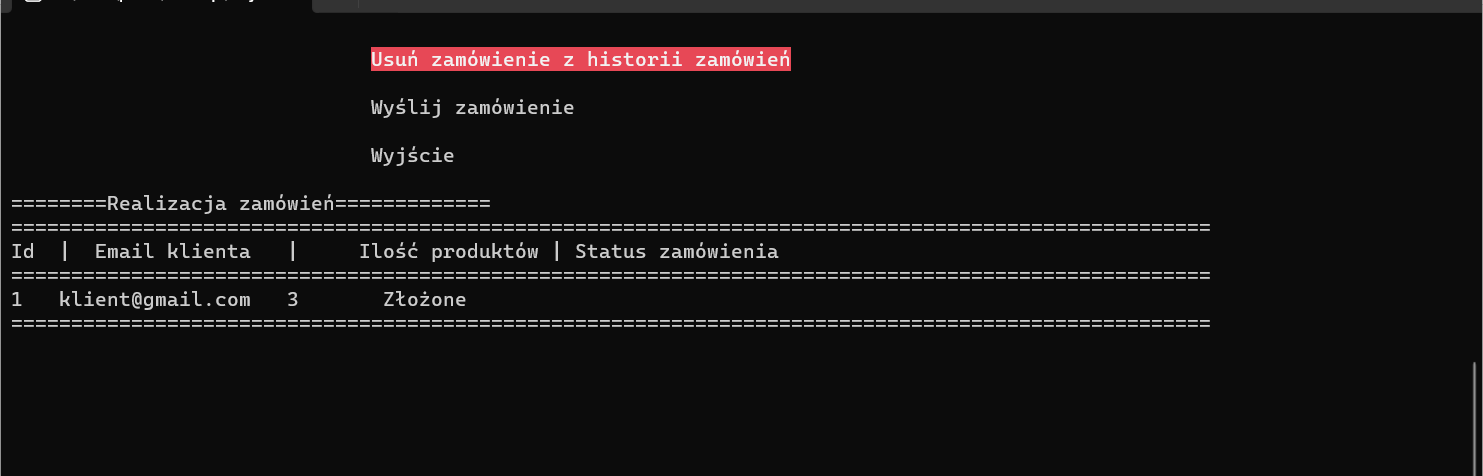
\includegraphics[width=15cm]{screeny/zamowienia_sprzedawca.png}
	\caption{\footnotesize Menu realizacja zamówień}
	\label{fig:plotend}
\end{figure}

\section{Klient}

Klient po poprawnym zalogowaniu do systemu, oprócz wiadomości powitalnej w lewym górnym rogu aplikacji ma do wyboru jedną z kilku opcji widocznych na \textit{Rysunku 5.7}. 

\begin{figure}[H]
	\centering
		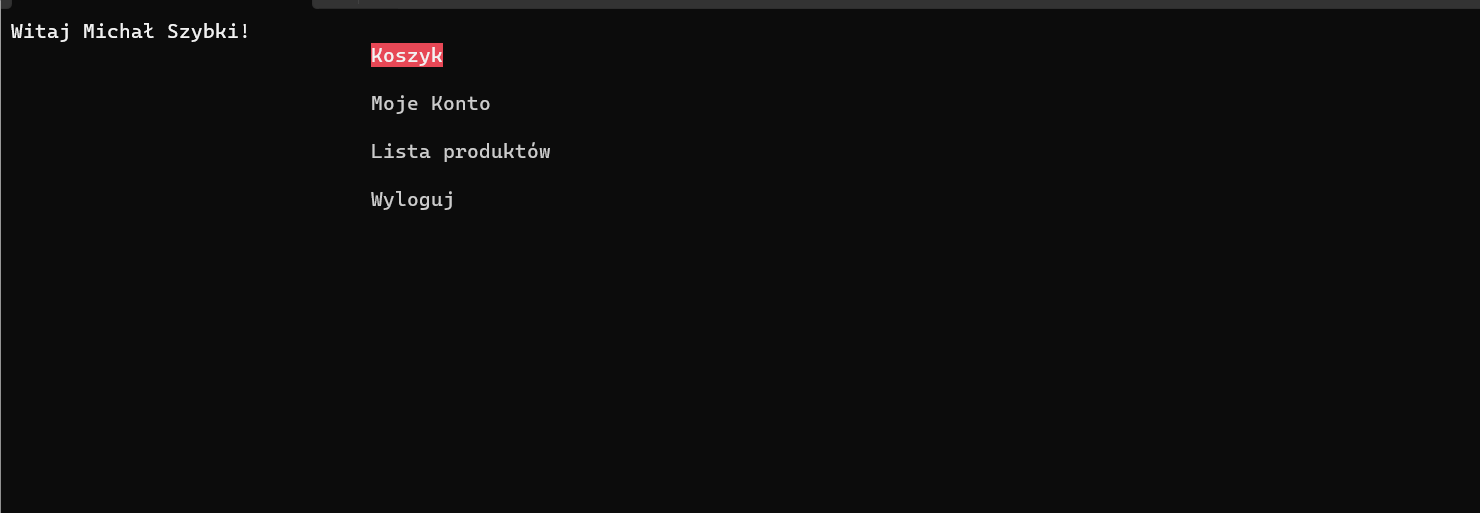
\includegraphics[width=15cm]{screeny/klient_menu.png}
	\caption{\footnotesize Menu klienta}
	\label{fig:plotend}
\end{figure}

Aby jednak w pierwszych dwóch pozycjach z menu wyświetliły się jakieś dane w przypadku nowo utoworzonego konta, należy najpierw przejść do opcji \textit{Lista produktów}. Aplikacja przekieruje użytkownika do widoku z dostępnymi produktami w sklepie, które następnie można sortować lub wyszukać po nazwie. 

\begin{figure}[H]
	\centering
		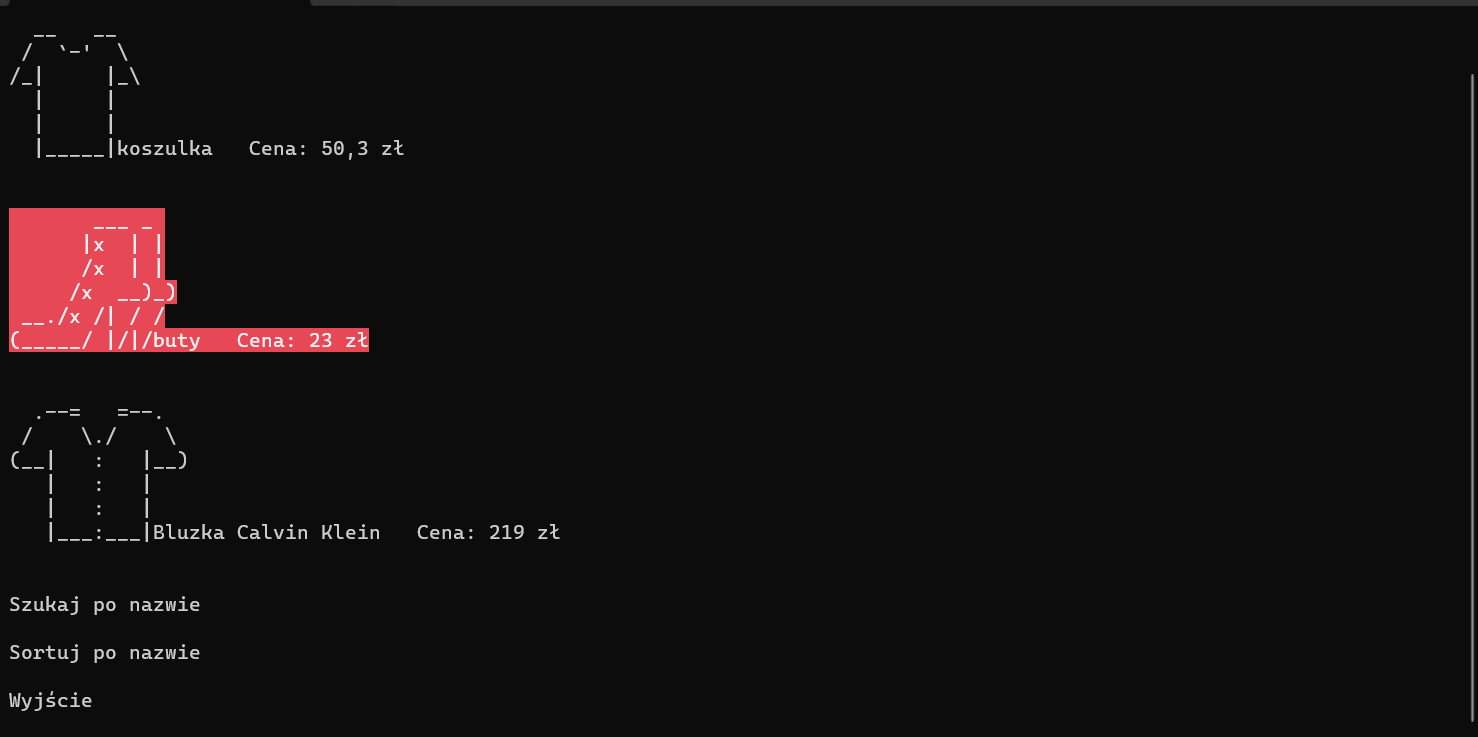
\includegraphics[width=15cm]{screeny/sklep_klient.png}
	\caption{\footnotesize Przeglądanie listy produktów w menu klienta}
	\label{fig:plotend}
\end{figure}

Rezultat wyszukiwania produktu po nazwie z frazą \textit{calvin} widoczny na \textit{Rysunku 5.9}.
	
\begin{figure}[H]
	\centering
		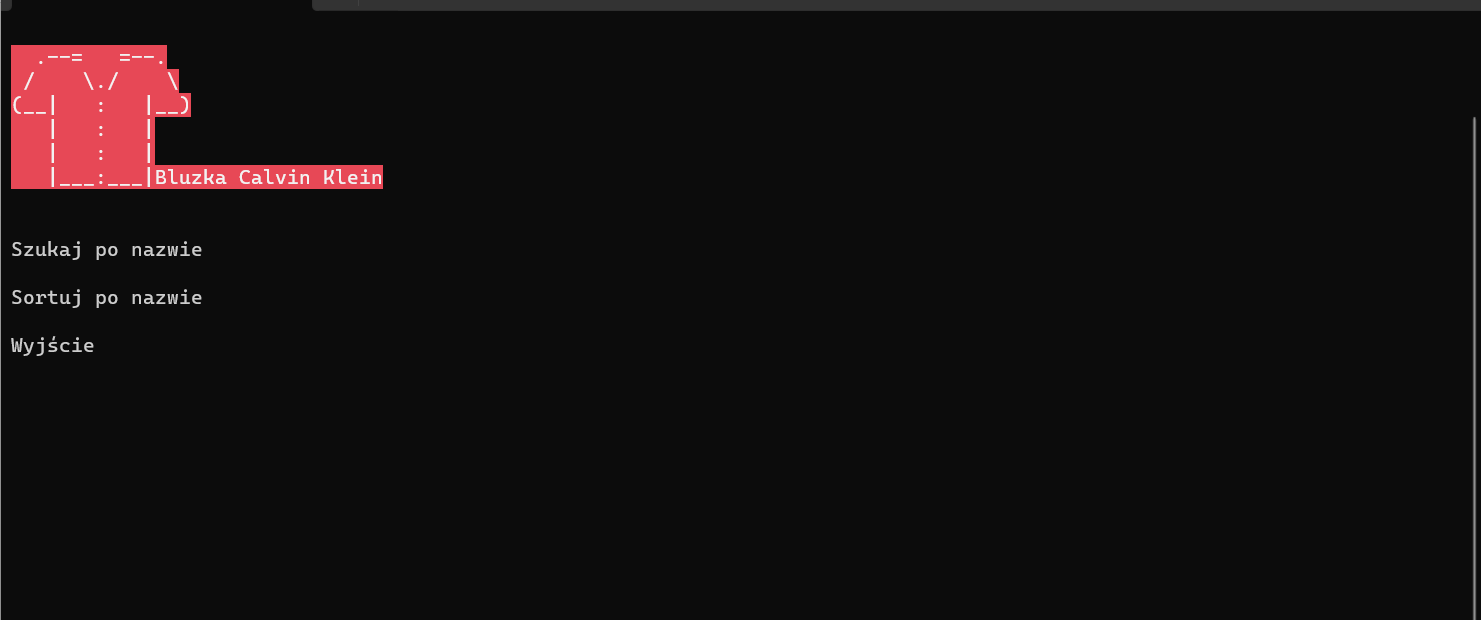
\includegraphics[width=15cm]{screeny/szukaj.png}
	\caption{\footnotesize Wyszukiwanie produktu po nazwie}
	\label{fig:plotend}
\end{figure}

Po wybraniu upatrzonego produktu, użytkownik może wybrać rozmiar oraz ilość sztuk. Jeśli wszystkie parametry zostały wybrane poprawnie, klient może dodać produkt do koszyka.

\begin{figure}[H]
	\centering
		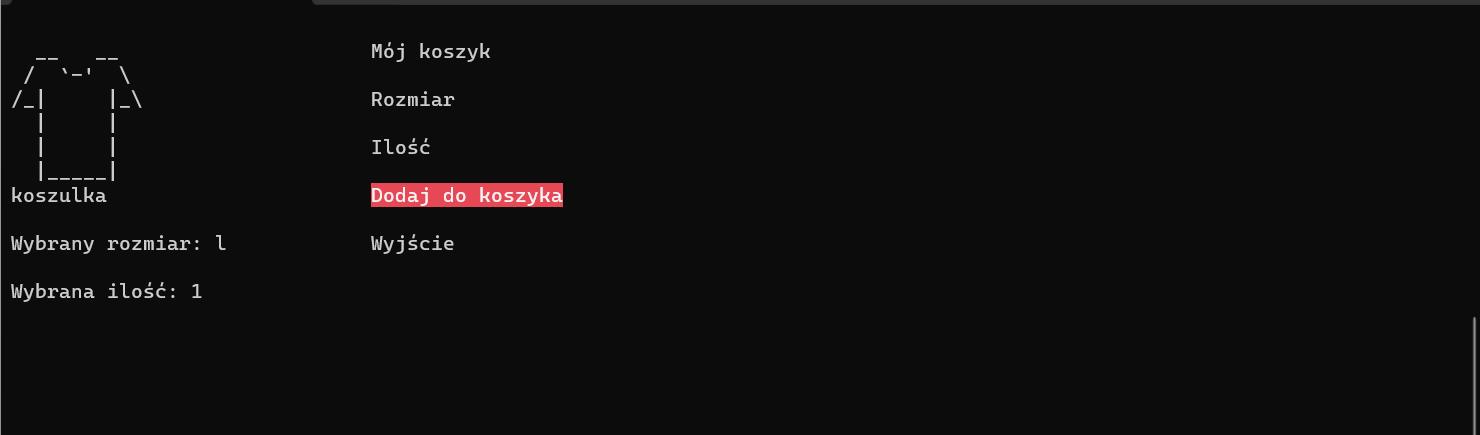
\includegraphics[width=15cm]{screeny/dodawanie_produktu_do_koszyka.png}
	\caption{\footnotesize Dodawanie produktu do koszyka}
	\label{fig:plotend}
\end{figure}

W koszyku znajdują się produkty, które klient dodał tam podczas działania aplikacji. Są one w nim widoczne tylko na czas działania aplikacji, czyli na czas sesji. W koszyku wyświetlana jest zsumowana liczba wszystkich produktów oraz zsumowana kwota zakupów. Klient widzi również dane do wysyłki. Są to dane podane podczas procesu rejestracji. W tym miejscu klient może jeszcze usunąć wybrany produkt z koszyka podając jego numer z listy w koszyku. Użytkownik może również wybrać opcję potwierdzenia zakupów, która utworzy zamówienie w systemie, aktualizując liczbę produktów w bazie danych oraz wyczyści koszyk klienta.

\begin{figure}[H]
	\centering
		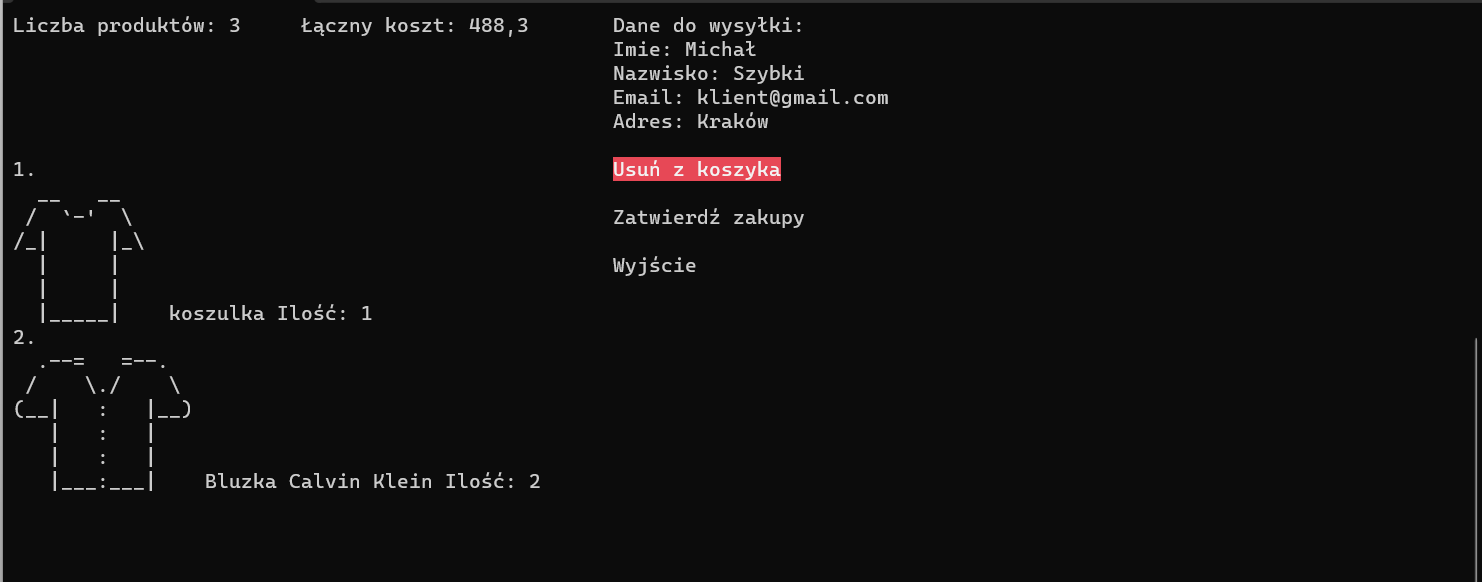
\includegraphics[width=15cm]{screeny/koszyk.png}
	\caption{\footnotesize Podgląd koszyka klienta}
	\label{fig:plotend}
\end{figure}

Ostatnią opcją, która nie została jeszcze opisana z menu klienta z \textit{Rysunku 5.7}, jest zakładka \textit{Moje konto}. Klient może tu zobaczyć swoje dane, w tym hasło. Co więcej, opcja ta wyświetla listę zamówień złożonych przez klienta w sklepie. Klient może wybrać konkretne zamówienie z listy i podejrzeć jakie produkty kupił w danym zamówieniu.

\begin{figure}[H]
	\centering
		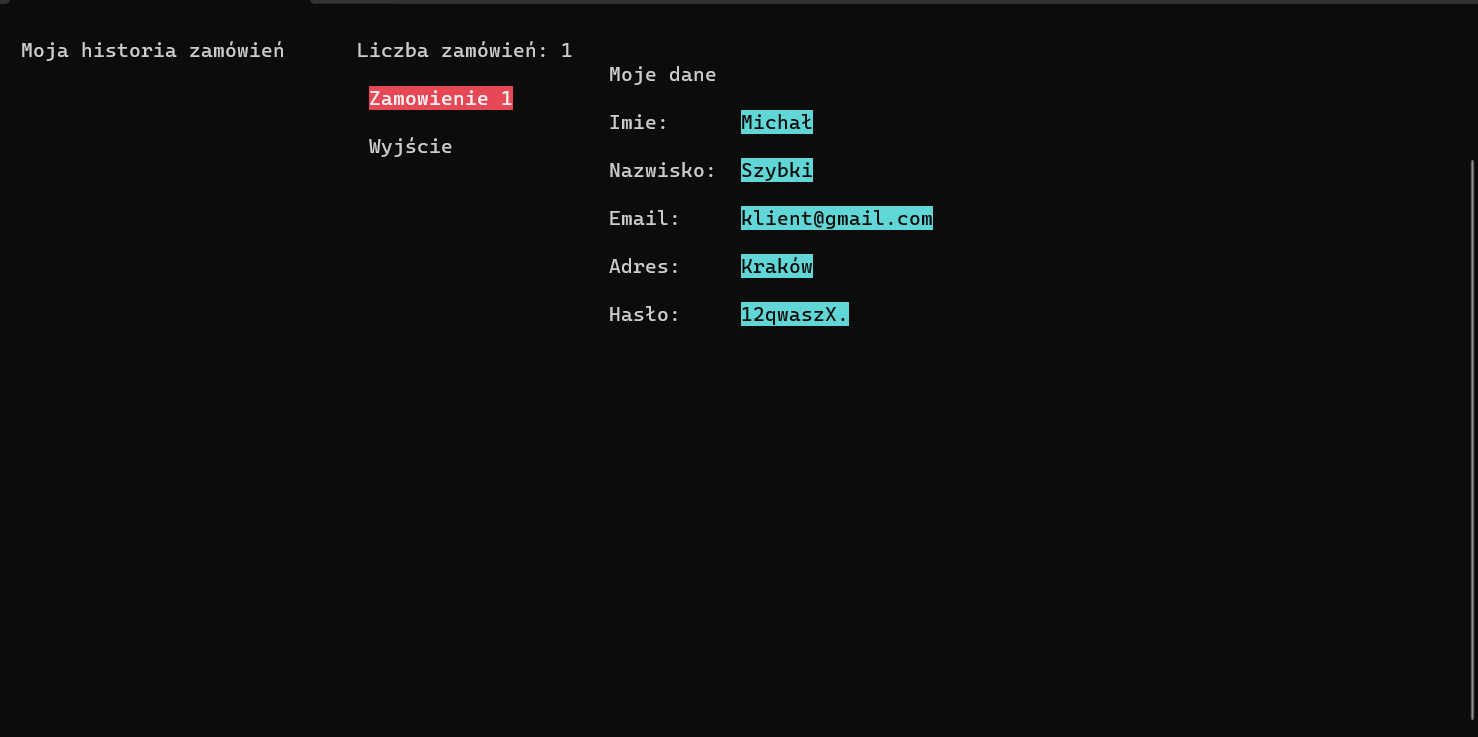
\includegraphics[width=15cm]{screeny/historia_klienta.png}
	\caption{\footnotesize Historia zamówień klienta oraz dane jego konta}
	\label{fig:plotend}
\end{figure}
\newpage
\chapter{Podsumowanie}
\section{Plany rozbudowy aplikacji}

Po zakończeniu pierwszej fazy projektu "Sklep", jedną ze ścieżek na rozwój aplikacji jest wprowadzenie nowych funkcjonalności oraz usprawnień mających na celu zwiększenie atrakcyjności, użyteczności i efektywności systemu.\newline

Aktualny system oparty jest na interfejsie konsolowym, jednak w planach jest wprowadzenie interfejsu graficznego (GUI), co znacznie poprawi wrażenia użytkownika. Przejście na interfejs z grafiką umożliwi bardziej intuicyjną nawigację oraz lepszą prezentację produktów. Jedną z możliwości jest stworzenie aplikacji okienkowej w rozwiązaniu WPF. Przy zmianie na tego typu aplikację, logika biznesowa pozostanie bez zmian. Trzeba ją jednak będzie dopasować do nowego interfejsu graficznego.\newline

Kolejną możliwością rozwoju jest przejście na wiele kategorii sprzedawanych produktów zwiększając asortyment lub podzial istniejących produktów na kategorie. Ułatwi to użytkownikom wyszukiwanie produktów oraz uporządkuje produkty w aplikacji.\newline

Podążając za trendem zaobserwowanym w innych aplikacjach tego typu, można utworzyć mechanizm systemu oceny i recenzji. Dodanie funkcji, która umożliwi klientom wystawianie ocen i recenzji produktów, nie tylko zwiększy zaufanie do sklepu, ale także dostarczy istotnych informacji zwrotnych dla sprzedawcy. Na podstawie tych danych system będzie mógł wyświetlać spersonalizowane sugestie produktów i je reklamować.

\section{Podsumowanie zrealizowanych prac}

Podczas tworzenia projektu "Sklep" w języku C\# w postaci programu konsolowego, głównym celem było stworzenie kompleksowego systemu obsługującego zarówno perspektywę sprzedawcy, jak i klienta. Dzięki zaimplementowanym funkcjonalnościom, aplikacja umożliwia sprawną obsługę procesów biznesowych, usprawnia zarządzanie asortymentem oraz zapewnia przyjazne i intuicyjne środowisko dla klientów dokonujących zakupów. Prace zostały zakończone sukcesem, a uzyskane rezultaty odpowiadają stawianym przed projektem celom.



\newpage

\begin{thebibliography}{6}
\addcontentsline{toc}{chapter}{Bibliografia}
%dodanie wpisu do spisu bibliograficznego


\bibitem{www} https://stackoverflow.com/ z dnia 29.12.2023
\bibitem{www} https://pasja-informatyki.pl/ z dnia 03.01.2024

\bibitem{ksiazka}Joseph Albahari, Ben Albahari, {\it C\# 9.0 in a Nutshell: The Definitive Reference},  O'Reilly Media, Sebastopol, Kalifornia, USA, 2021.
\bibitem{ksiazka}Bartłomiej Filipek, {\it Programowanie w C\#. Teoria i praktyka}, Helion, Gliwice 2019.
\bibitem{ksiazka}Andrzej Ślęzak, Wojciech Ślęzak, {\it C\# Od Podstaw. Wydanie V}, Helion, Gliwice 2018.
\end{thebibliography}
\newpage


\end{document}
